\section{Results}
\subsection{Functional validation before policy learning}
The manual LoRA implementation was exercised with the Qwen model on CPU/float32. It replaced and merged \ReplacedCount{} linear layers: seven targeted projections in each of 24 transformer blocks. The adapters introduced \TrainableCount{} trainable parameters out of \TotalCount{} combined parameters (\TrainableRatio{}). A forward pass and merging completed, and nine lightweight behavior/interface tests passed. These checks establish implementation behavior; the functional entry point contains no language-model optimizer loop. The six implementation responsibilities are summarized in Appendix~\ref{app:implementation}.

\subsection{A saved policy and a paired arithmetic improvement}\label{sec:policy-results}
The independent 16-prompt save/reload check passed before the full A10 experiment. The full run then started from the original base model and completed 512 prompts / \PPORolloutSteps{} batches with exit code 0. All recorded scalars and saved adapter values were finite. Nonzero B tensors were found in all \PPOBTensors{} Actor and \PPOCriticBTensors{} Critic adapter tensors.

The Actor was actually reloaded on the GPU and passed finite forward and generation checks. The Critic adapter passed checksum, finite-value and nonzero-update checks, but was not reloaded. These statements distinguish saved-weight inspection from executable model recovery.

\par\noindent\begin{minipage}{\linewidth}
\tabcaption{tab:paired}{Matched BF16 development-validation outcomes. Both sides use the same 128 questions, greedy decoding, length limit and scoring code.}
\begin{tabularx}{\linewidth}{@{}Y P{39mm}P{39mm}@{}}
\toprule
\tablehead Measurement & Base policy & After PPO\\
\midrule
Correct first-line answers & \PPOBaselineCorrect{}/\PPOValidationN & \PPOTrainedCorrect{}/\PPOValidationN\\
Accuracy & \PPOBaselineAccuracy & \PPOTrainedAccuracy\\
Change & --- & \PPODelta{} percentage points\\
\bottomrule
\end{tabularx}
\end{minipage}\par


\par\noindent\begin{minipage}{\linewidth}
\begin{center}
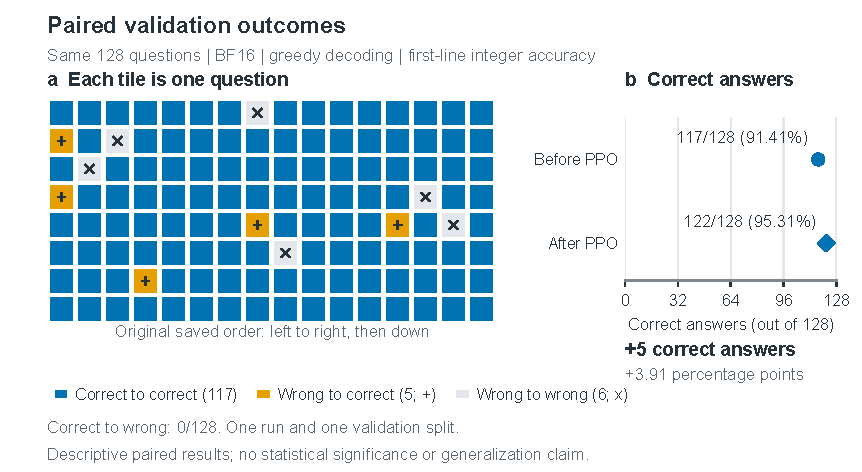
\includegraphics[width=146mm]{../../figures/paired_validation_outcomes.pdf}
\end{center}
\figcaption{fig:paired}{The saved responses are matched question by question. There are 117 correct-to-correct outcomes, five wrong-to-correct outcomes, six wrong-to-wrong outcomes and no correct-to-wrong outcomes. Every outcome is recomputed from the original responses; tiles or marks represent questions rather than repeated experimental runs.}
\end{minipage}\par


The improvement is a net five corrected questions. Examples include $15+23$, changing from 48 to 38, and $45+48$, changing from 133 to 93. Errors remain: $2+33$ changes from 34 to 36, with neither answer correct. This pattern supports a narrow task-level improvement while also showing why a higher aggregate score is not complete arithmetic reliability. The historical T4 baseline of 118/128 uses FP32 and belongs to another run; it is excluded from Table~\ref{tab:paired}.

\subsection{Training dynamics: useful signals with different meanings}
\par\noindent\begin{minipage}{\linewidth}
\begin{center}
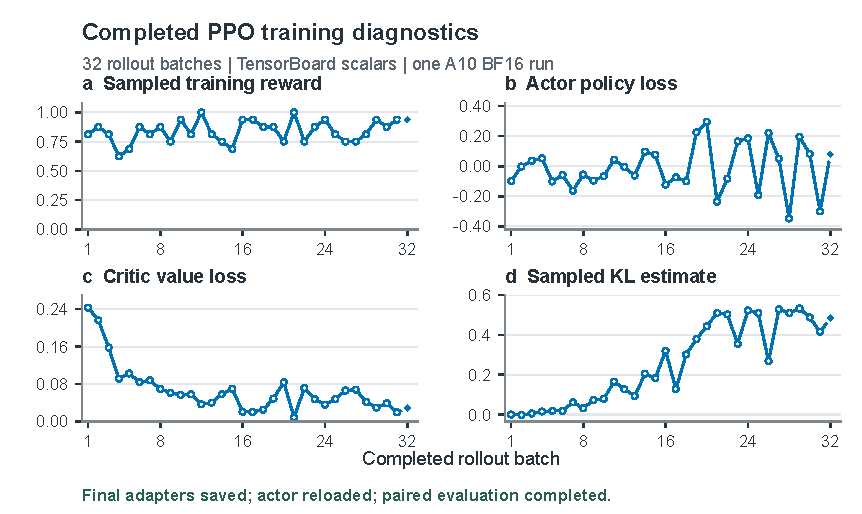
\includegraphics[width=146mm]{../../figures/ppo_training_success.pdf}
\end{center}
\figcaption{fig:ppo-curves}{All 32 measured rollout-batch values of the successful A10 run, without smoothing. Each batch contains 16 prompts. KL is a sampled estimate: its small negative value near the start does not imply a negative theoretical KL divergence.}
\end{minipage}\par


Mean training reward rises from 0.8125 in the first batch to 0.9375 in the last, but ranges between 0.625 and 1.0. Each batch contains different questions and sampled responses, so the endpoints are not a paired estimate of learning. The paired greedy validation in Figure~\ref{fig:paired} provides the direct performance comparison.

Critic loss decreases from approximately 0.2431 to 0.0283, consistent with better fit to the sampled return targets. Actor loss changes sign and fluctuates; it is the signed clipped objective, not a measure of the fraction of correct answers. Estimated KL reaches about 0.485 in the last batch, showing increasing departure from the fixed reference. Neither a lower value loss nor a larger policy departure by itself establishes a task-performance gain.

The logged mean response length changes from 29.125 to 15.5625 tokens between the first and last batches. Some corrected validation responses are shorter, but other answers still continue with additional questions. These observations are compatible with the first-line reward rule; no ablation isolates response length as the cause of improvement.

\smallheading{What the execution evidence adds}
The saved-weight checks close a practical gap left by an earlier run that completed its rollout loop but failed at final serialization. Completion here is established jointly by exit code, full scalar coverage, finite/nonzero adapters, actual Actor reloading and saved paired responses. An isolated progress bar would establish much less. Appendix~\ref{app:recovery} retains both the earlier failure and the later export-manifest ambiguity.

\subsection{Program search: the winner arrived during initialization}\label{sec:program-results}
Seven proposal records are present in the final online export. Five passed the evaluator, one failed implementation with a Python syntax error, and one had no evaluation yet. Only completed valid evaluations enter Table~\ref{tab:online} and Figure~\ref{fig:online}. Generation 0 denotes initialization; island indices are zero-based.

\par\noindent\begin{minipage}{\linewidth}
\tabcaption{tab:online}{Valid online evaluations on 31 October 2026. Times are UTC+08:00; full-precision records remain in the original CSV.}
\begin{tabularx}{\linewidth}{@{}P{28mm}P{13mm}P{14mm}P{30mm}Y@{}}
\toprule
\tablehead Candidate & Gen. & Island & Sum of radii & Time\\
\midrule
\code{fe0aad416d4f} & 0 & 0 & 2.473873492 & 12:46:55\\
\code{4705b8e92e1b} & 0 & 1 & \key{2.620013807} & 13:08:21\\
\code{d3fb7a9f0bab} & 0 & 1 & 2.464972339 & 13:10:19\\
\code{34836c89e4f0} & 1 & 1 & 2.616027976 & 13:18:13\\
\code{a15ea29f0ceb} & 1 & 0 & 2.514353475 & 13:18:47\\
\bottomrule
\end{tabularx}
\end{minipage}\par


\par\noindent\begin{minipage}{\linewidth}
\begin{center}
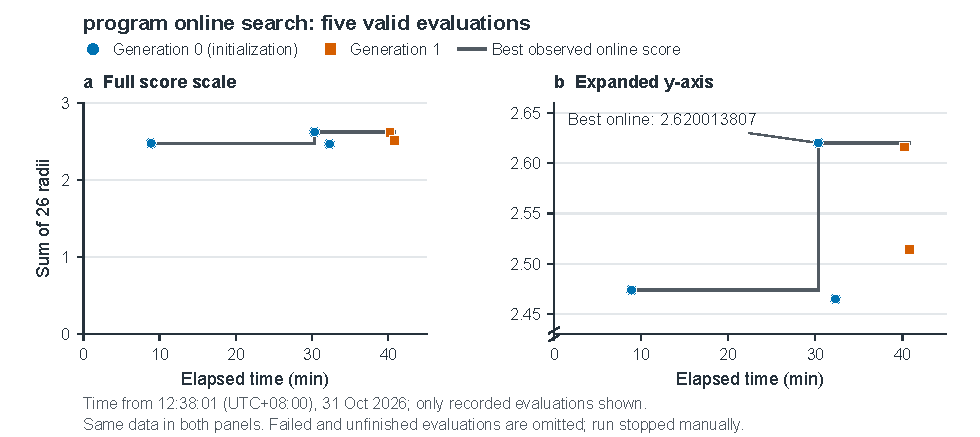
\includegraphics[width=166mm]{../../program_search/figures/online_progress.pdf}
\end{center}
\figcaption{fig:online}{The same five online scores at full scale and with an explicitly expanded y-axis. Circles denote initialization and squares generation 1; the step line is the running best. Failed or missing evaluations are not plotted as zero, and the line is not extended beyond observed evaluations.}
\end{minipage}\par


For valid candidates observed by time $t$, the incumbent is
\begin{equation}
S_t^\star=\max_{a\in\mathcal V_t}S(a),\qquad\mathcal V_t\ne\varnothing.
\end{equation}
The best online score is 2.62001380699489, from initial candidate \code{4705b8e92e1b}. A generation-1 child improves its own parent from 2.473873492 to 2.514353475, but neither observed child beats the global incumbent. Local parent improvement and improvement of the overall search are therefore different events. The run demonstrates generation, execution and selection; its short, manually stopped trajectory establishes neither convergence nor an optimum.

\subsection{Independent geometry: a separate result, not a replacement score}
The selected program tries eight deterministic starting layouts and uses SLSQP to adjust centers and radii jointly. With centers fixed, its radius allocation is a linear program:
\begin{equation}
\max_{\boldsymbol r}\sum_i r_i\quad\text{subject to}\quad
0\le r_i\le b_i,\quad r_i+r_j\le d_{ij}\quad(i<j),
\end{equation}
where $b_i=\min(x_i,y_i,1-x_i,1-y_i)$ and $d_{ij}=\|\boldsymbol c_i-\boldsymbol c_j\|_2$. A final conservative radius repair reduces numerical violations. Optimal radii for fixed centers do not establish a globally optimal layout.

\par\noindent\begin{minipage}{\linewidth}
\begin{center}
\begin{minipage}[t]{0.47\linewidth}\centering
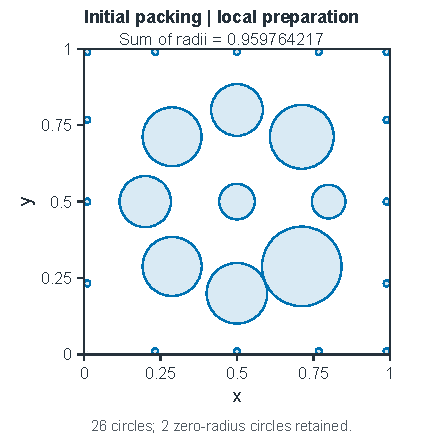
\includegraphics[width=75mm]{../../program_search/figures/initial_packing.pdf}\\
{\small (a) Official initial constructor}
\end{minipage}\hfill
\begin{minipage}[t]{0.47\linewidth}\centering
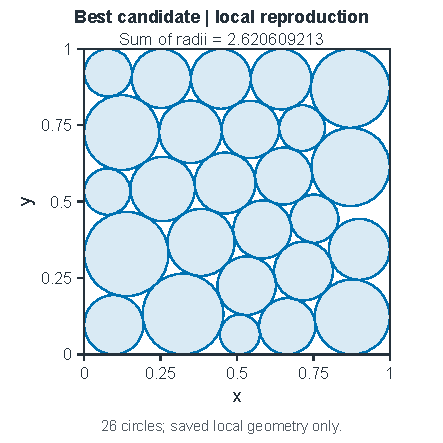
\includegraphics[width=75mm]{../../program_search/figures/online_best_reproduced.pdf}\\
{\small (b) Selected program, re-executed locally}
\end{minipage}
\end{center}
\figcaption{fig:geometry}{Two separate local geometry records. Panel (a) has sum 0.9597642169962063; panel (b) has sum 2.6206092130170973. The plots preserve the original saved centers, radii and equal scale. Panel (b) is not the server's original geometry and does not replace its online score.}
\end{minipage}\par


Unmodified local execution of the selected source took about 4.76 seconds using Python 3.14.2, NumPy 2.4.4 and SciPy 1.17.1. The original geometry method accepted all 26 circles. Minimum boundary and pair gaps were approximately $1.38\times10^{-12}$ and $1.02\times10^{-12}$: positive in the saved calculation, but numerically small.

The local sum, 2.6206092130170973, exceeds the online record by approximately 0.000595406. Runtime or numerical differences are plausible explanations; their cause was not isolated. The online experiment result remains 2.62001380699489. Likewise, the local initial-constructor value is not a same-run online baseline, so no online percentage gain is computed from it.
